\documentclass{amsc}          %此模板需调用宏包amsc.cls, 请确保此宏包与tex文件在同一文件夹下
\numberwithin{equation}{section} % 公式编号会随着Section而变动,如(1.1),(1.2),(2.1)...,如果不便使用,您可以将这个命令删去
\usepackage[colorlinks,
            linkcolor=red,
            anchorcolor=blue,
            citecolor=green
            ]{hyperref}
\usepackage{tikz}
\usepackage{amsmath}

\begin{document}

\Volume{201x}{1}{0}{0}               % 年、月、卷、期
\PageNum{1}                                  % 起始页码
\PaperID{0583-1431(20xx)0x-0xxx-0x}   % 文章编号
\DocumentCode{A}                              % 文献标识码
\EditorNote{收稿日期:\ 200x-xx-xx;\ 接受日期:\ 200x-xx-xx}  % 脚注

%%%%%%%%%%%%%%%%%%%%%%%%%%%%%%%%%%%%%%%%%%%%%%%%%%%%%%%%%%%%%%%%%%%%%%%%%%%%
%%%%%  作者从下面开始填写各项内容,本刊的标点符号均使用英文标点,您可以在编译前设置标点形式

\EditorNote{基金项目: }            %如 基金项目:国家自然科学基金资助项目(10171074),如没有基金项目请删去此行

\TitleMark{惠慧:栅格覆盖的计数表示及超矩阵的行列式}  % 页眉, 如有多位作者,请写为 第一作者姓名等: 论文标题缩写

\BeginTitle

\Title{栅格覆盖的计数表示及超矩阵的行列式}

\Author{惠慧}
 {南京大学\  南京\ 210093\\
E-mail: huih1984@outlook.com}

\Abstract{在文章\cite{Kly} 中,$Kasteleyn$($Fisher$和$Temperley$ 同时独立)开创性研究了多米诺覆盖计数问题,这后来被称为$FKT$算术,它在平面图上的全息算法中得到广泛应用。本文作者这里提出如何将 $dimer$覆盖问题泛化到$1 \times 2N$ 长方块覆盖,文章主要讨论$1 \times 4$ 长方块的覆盖问题,从而可以自然推广到$1 \times 2N$ 的覆盖计算,之所以奇数形式的覆盖问题不讨论是其不具有自然泛化的特性,而在偶数的情况下,计数表达方法存在自然的形式泛化。本文的一个关键结果即在内维数为$4$ 的情况下,延拓矩阵、行列式以及$pf$ 定义,得到 $det(A)=pf^{4}(A)$, 从而进一步得出内维数为$2N$ 时,$det(A)=pf^{2N}(A)$,从形式上看,这个结果是$Cayley$给出的$det(A)=pf^{2}(A)$证明的一个完美推广!}

\Keywords{双重维数矩阵; 内维数; 多米诺覆盖; 外积; $pf$;}


\ETitle{counting number of lattice tilings and hyperdeterminant} %英文标题

\EAuthor{Hui \uppercase{Hui}} % 作者姓名的拼音,名在前,姓在后
{Nanjing University, Nanjing $100190$, P. R. China \\            % 如 Academy of Mathematics and Systems Science, Chinese Academy of Sciences, Beijing $100190$, P. R. China \\
E-mail\,$:$ huih1984@outlook.com}

\EAbstract{Kasteleyn(Fisher \& Temperley independently) start the question about counting number of domino tiling, which is called as FKT algorithm later, The FKT algorithm has seen extensive use in holographic algorithms on planar graphs. Author introduce a new question how to extend the counting number about $1 \times 2N$ pane tiling? Author focus the question on $ 1 \times 4$, because the counting method can easy be extended to $1 \times 2N$, the odd case is not be discussed because of that is not easy to extend. The article's main result is $det(A)=pf^{4}(A)$, when inner dimension is 4, and matrix, determinant is extended. Similarly, when inner dimension is $2N$, $det(A)=pf^{2N}(A)$,the result is perfect extended as Cayley's formula in form!}
\EKeywords{double dimension matrix; inner dimension; domino tiling; wedge product; pf;}

\EndTitle


\Section{引言}
关于$dimer$覆盖数的计算问题,起源于统计力学和分子化学,物理学家们提出的原始问题是双原子分子被吸附在一个平面上,形成一个单层,那么有多少种排列方式?\cite{Kly}的文章给出了$dimer$在$m \times n$ 的块状上和环面上的覆盖数的计算公式,并且$dimer$覆盖问题被泛化到所有平面图\cite{Kly2}。但是另外一类问题就是$trimer,tetramer$等覆盖计数问题没有更多涉及,用$1\times n$ 覆盖的文章有\cite{MA},但是文章只讨论了被覆盖为$9 \times n$ 的计算公式,本文关注$1 \times 2n$ 骨牌覆盖一般性的计数问题。
%数学公式在推广到更高阶的情形,情况往往变得复杂,比如方程解的问题,在小于五次时,有比较简单根式形式,而高于五次的方程一般而言没有根式解,给出深刻的约束条件,高阶方程的根式解依然存在,这个
% 数学历史上的著名问题给人深深的哲思启发。理论的推广几乎总是去除局限的部分,余下的情形就可以拓展开来,发现更多的现象和本质,本文接下来就讨论$1 \times 4$骨牌覆盖数的计算公式。

%很容易得到类似于$pf$的表达形式,进而作者一直在寻找转换成矩阵表达形式,之所以这么做是因为从形式上来看,这种矩阵的存在完全符合数学符号的形式美,经过一番努力,终于找到了相应的矩阵形式。而这种拓展的矩阵形式本身却更有耐人寻味的结构美,作者没有见过有什么文献对这种形式的矩阵有深入的研究,这里作者只得出了一些少量的结果,作者能力有限,希望有更多的研究者参与其中来研究这种矩阵。

\Section{表示方法}

\begin{center}

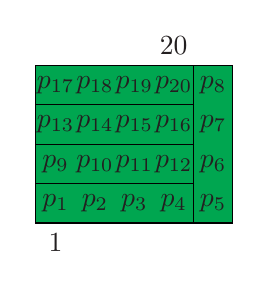
\begin{tikzpicture}
\selectcolormodel{cmyk}
\node at (.25,-.25) {$1$};
\path [fill=black](0,0) rectangle (2,.5);
\draw [fill=green](0,0) rectangle (2,.5);
\node at (.25,.25) {$p_{1}$};
\node at (.75,.25) {$p_{2}$};
\node at (1.25,.25) {$p_{3}$};
\node at (1.75,.25) {$p_{4}$};
\path [fill=black] (0,0.5)rectangle(2,1);
\draw [fill=green] (0,0.5)rectangle(2,1);
\node at (.25,.75) {$p_{9}$};
\node at (.75,.75) {$p_{10}$};
\node at (1.25,.75) {$p_{11}$};
\node at (1.75,.75) {$p_{12}$};
\path [fill=black] (0,1)rectangle(2,1.5);
\draw [fill=green] (0,1)rectangle(2,1.5);
\node at (.25,1.25) {$p_{13}$};
\node at (.75,1.25) {$p_{14}$};
\node at (1.25,1.25) {$p_{15}$};
\node at (1.75,1.25) {$p_{16}$};
\path [fill=black] (2,0)rectangle(2.5,2);
\draw [fill=green] (2,0)rectangle(2.5,2);
\node at (2.25,.25) {$p_{5}$};
\node at (2.25,.75) {$p_{6}$};
\node at (2.25,1.25) {$p_{7}$};
\node at (2.25,1.75) {$p_{8}$};
\path [fill=black] (0,1.5)rectangle(2,2);
\draw [fill=green] (0,1.5)rectangle(2,2);
\node at (.25,1.75) {$p_{17}$};
\node at (.75,1.75) {$p_{18}$};
\node at (1.25,1.75) {$p_{19}$};
\node at (1.75,1.75) {$p_{20}$};
\node at (1.75,2.25) {$20$};
\end{tikzpicture}
\end{center}
采用$Kasteleyn^{[1]}$相同的表示方法,$C=(p_{1},p_{2},p_{3},p_{4})(p_{5},p_{6},p_{7},p_{8})...(p_{N-3},p_{N-2},p_{N-1},p_{N})$.\\
    其中$(p_{j},p_{j+1},p_{j+2},p_{j+3})$为一个长方块的四个连续坐标。

    \begin{equation}\label{a}p_{1}<p_{2}<p_{3}<p_{4},p_{5}<p_{6}<p_{7}<p_{8}
   ,...,p_{N-3}<p_{N-2}<p_{N-1}<p_{N}\end{equation}

   \begin{equation}\label{b}p_{1}<p_{5}<...<p_{N-3}\end{equation}

   \begin{equation}a_{(i,j;i+1,j;i+2,j;i+3,j)}=1,1\leq i \leq m-3,1\leq j\leq n\end{equation}
   \begin{equation}a_{(i,j;i,j+1;i,j+2;i,j+3)}=1,1\leq i \leq m,1\leq j\leq n-3\end{equation}
   \begin{equation}a_{(i,j;i^{'},j^{'};i^{''},j^{''};i^{'''},j^{'''})}=0,other \end{equation}

   \begin{equation}\label{c}pf(A_{4})=\sum\limits_{\sigma=p_{1}p_{2}...p_{N}satisfy(1)(2)}sgn\sigma a_{p_{1}p_{2}p_{3}p_{4}}a_{p_{5}p_{6}p_{7}p_{8}}...a_{p_{N-3}p_{N-2}p_{N-1}p_{N}}\end{equation}

   对应的矩阵记为$A_{4}=(a_{ijkl})$,满足$a_{jikl}=-a_{ijkl}$,$i,j,k,l$的任意一个序关系都满足逆序数正负号。
   这样得到的表达式$\ref{c}$,仍然称为$pf$。


\Section{$pf \rightarrow det$的转换}

\begin{definition} 矩阵的内维数和外维数:

$\begin{bmatrix}
a_{i_{1}i_{2}...i_{n}}\end{bmatrix}_{m}$为$n$个下指标构成的多维矩阵,每个指标取值为$1,2,\cdots,m$,则$n$称为内维数,$m$称为外维数。此文只考虑$n$为4的情形。
\end{definition}

\begin{definition} 矩阵行列式:
\end{definition}

将$[a_{ijkl}]$表示成矩阵的矩阵形式,内部子矩阵的指标为$i,j$,外部矩阵指标为$k,l$,行列式$det$满足如下性质:
\newcounter{Lcount}
\begin{list}{\Roman{Lcount}}
{\usecounter{Lcount}
\setlength{\rightmargin}{\leftmargin}}
%\scriptsize
\item
系数性质,行列式乘以系数k,与在某个指标中的固定取值上乘以k所得矩阵的行列式相等。如取$l=1$如下:
\begin{align*}
s*det
  \begin{bmatrix}
  \begin{bmatrix}
  \  a_{1111}&\  a_{2111}&\cdots&\  a_{n111}\\
 \  a_{1211}&\  a_{2211}&\cdots&\  a_{n211}\\
  \vdots&\vdots&\ddots &\vdots& \\
\  a_{1n11}&\  a_{2n11}&\cdots&\  a_{nn11}\\
 \end{bmatrix}&
\cdots&
\begin{bmatrix}
\  a_{11n1}&\  a_{21n1}&\cdots&\  a_{n1n1}\\
\  a_{12n1}&\  a_{22n1}&\cdots&\  a_{n2n1}\\
  \vdots&\vdots&\ddots &\vdots& \\
\  a_{1nn1}&\  a_{2nn1}&\cdots&\  a_{nnn1}\\
\end{bmatrix}\\
\vdots&\vdots&\vdots\\
\begin{bmatrix}
\  a_{111n}& \  a_{211n}&\cdots&\  a_{n11n}\\
\  a_{121n}& \  a_{221n}&\cdots&\  a_{n21n}\\
  \vdots&\vdots&\ddots &\vdots& \\
\  a_{1n1n}& \  a_{2n1n}&\cdots& \  a_{nn1n}\\
\end{bmatrix}&
\cdots&
\begin{bmatrix}
\  a_{11nn}& \  a_{21nn}&\cdots&\  a_{n1nn}\\
\  a_{12nn}& \  a_{22nn}&\cdots&\  a_{n2nn}\\
  \vdots&\vdots&\ddots &\vdots& \\
\  a_{1nnn}& \  a_{2nnn}&\cdots&\  a_{nnnn}\\
\end{bmatrix}
\end{bmatrix}\\
\\
=det
  \begin{bmatrix}
  \begin{bmatrix}
 sa_{1111}& sa_{2111}&\cdots&sa_{n111}\\
 sa_{1211}& sa_{2211}&\cdots&sa_{n211}\\
  \vdots&\vdots&\ddots &\vdots& \\
sa_{1n11}& sa_{2n11}&\cdots&sa_{nn11}\\
 \end{bmatrix}&
\cdots&
\begin{bmatrix}
sa_{11n1}& sa_{21n1}&\cdots&sa_{n1n1}\\
sa_{12n1}& sa_{22n1}&\cdots&sa_{n2n1}\\
  \vdots&\vdots&\ddots &\vdots& \\
sa_{1nn1}& sa_{2nn1}&\cdots&sa_{nnn1}\\
\end{bmatrix}\\
\vdots&\vdots&\vdots\\
\begin{bmatrix}
\  a_{111n}& \  a_{211n}&\cdots&\  a_{n11n}\\
\  a_{121n}& \  a_{221n}&\cdots&\  a_{n21n}\\
  \vdots&\vdots&\ddots &\vdots& \\
\  a_{1n1n}& \  a_{2n1n}&\cdots&\  a_{nn1n}\\
\end{bmatrix}&
\cdots&
\begin{bmatrix}
\  a_{11nn}& \  a_{21nn}&\cdots& \  a_{n1nn}\\
\  a_{12nn}& \  a_{22nn}&\cdots&\  a_{n2nn}\\
  \vdots&\vdots&\ddots &\vdots& \\
\  a_{1nnn}& \  a_{2nnn}&\cdots& \  a_{nnnn}\\
\end{bmatrix}
\end{bmatrix}
 \end{align*}
 \item
 符号性质,某个指标下的任意两列交换位置,行列式正负号互换,例如下:
\begin{align*}
det
  \begin{bmatrix}
\vdots&\vdots&\vdots\\
 \begin{bmatrix}
 a_{111\xi}& a_{211\xi}&\cdots&a_{n11\xi}\\
 a_{121\xi}& a_{221\xi}&\cdots&a_{n21\xi}\\
  \vdots&\vdots&\ddots &\vdots&\\
a_{1n1\xi}& a_{2n1\xi}&\cdots&a_{nn1\xi}\\
\end{bmatrix}&
\cdots&
\begin{bmatrix}
  a_{11n\xi}& a_{21n\xi}&\cdots&a_{n1n\xi}\\
  a_{12n\xi}& a_{22n\xi}&\cdots&a_{n2n\xi}\\
  \vdots&\vdots&\ddots &\vdots& \\
 a_{1nn\xi}& a_{2nn\xi}&\cdots&a_{nnn\xi}\\
 \end{bmatrix}\\
\vdots&\vdots&\vdots\\
\begin{bmatrix}
  a_{111\eta}& a_{211\eta}&\cdots&a_{n11\eta}\\
  a_{121\eta}& a_{221\eta}&\cdots&a_{n21\eta}\\
  \vdots&\vdots&\ddots &\vdots& \\
   a_{1n1\eta}& a_{2n1\eta}&\cdots&a_{nn1\eta}\\
   \end{bmatrix}&
\cdots&
\begin{bmatrix}
  a_{11n\eta}& a_{21n\eta}&\cdots&a_{n1n\eta}\\
  a_{12n\eta}& a_{22n\eta}&\cdots&a_{n2n\eta}\\
  \vdots&\vdots&\ddots &\vdots& \\
   a_{1nn\eta }& a_{2nn\eta}&\cdots&a_{nnn\eta}\\
   \end{bmatrix}\\
\vdots&\vdots&\vdots\\
    \end{bmatrix}\\
=-det
  \begin{bmatrix}
\vdots&\vdots&\vdots\\
 \begin{bmatrix}
   a_{111\eta}& a_{211\eta}&\cdots&a_{n11\eta}\\
   a_{121\eta}& a_{221\eta}&\cdots&a_{n21\eta}\\
  \vdots&\vdots&\ddots &\vdots& \\
   a_{1n1\eta}& a_{2n1\eta}&\cdots&a_{nn1\eta}\\
   \end{bmatrix}&
\cdots&
\begin{bmatrix}
  a_{11n\eta}& a_{21n\eta}&\cdots&a_{n1n\eta}\\
  a_{12n\eta}& a_{22n\eta}&\cdots&a_{n2n\eta}\\
  \vdots&\vdots&\ddots &\vdots& \\
  a_{1nn\eta }& a_{2nn\eta}&\cdots&a_{nnn\eta}\\
  \end{bmatrix}\\
\vdots&\vdots&\vdots\\
 \begin{bmatrix}
   a_{111\xi}& a_{211\xi}&\cdots&a_{n11\xi}\\
   a_{121\xi}& a_{221\xi}&\cdots&a_{n21\xi}\\
  \vdots&\vdots&\ddots &\vdots&\\
a_{1n1\xi}& a_{2n1\xi}&\cdots&a_{nn1\xi}\\
\end{bmatrix}&
\cdots&
\begin{bmatrix}
  a_{11n\xi}& a_{21n\xi}&\cdots&a_{n1n\xi}\\
  a_{12n\xi}& a_{22n\xi}&\cdots&a_{n2n\xi}\\
  \vdots&\vdots&\ddots &\vdots&\\
  a_{1nn\xi}& a_{2nn\xi}&\cdots&a_{nnn\xi}\\
  \end{bmatrix}\\
\vdots&\vdots&\vdots\\
    \end{bmatrix}
\end{align*}
 \item
 加法性质,任意一个列中和式可以分解,例如下
%\begin{align*}
 $$det\begin{bmatrix}
 \begin{bmatrix}\begin{smallmatrix}
 a_{1111} + a_{1111}^{'}& a_{2111} + a_{2111}^{'}&\cdots&a_{n111} + a_{n111}^{'}\\
 a_{1211} + a_{1211}^{'}& a_{2211} + a_{2211}^{'}&\cdots&a_{n211} + a_{n211}^{'}\\
  \vdots&\vdots&\ddots &\vdots& \\
a_{1n11} + a_{1n11}^{'}& a_{2n11} + a_{2n11}^{'}&\cdots&a_{nn11} + a_{nn11}^{'}\\
\end{smallmatrix}\end{bmatrix}&
\cdots&
\begin{bmatrix}\begin{smallmatrix}
  a_{11n1} + a_{11n1}^{'}& a_{21n1} + a_{21n1}^{'}&\cdots&a_{n1n1} + a_{n1n1}^{'}\\
a_{12n1} + a_{12n1}^{'}& a_{22n1} + a_{22n1}^{'}&\cdots&a_{n2n1} + a_{n2n1}^{'}\\
  \vdots&\vdots&\ddots &\vdots& \\
 a_{1nn1} + a_{1nn1}^{'}& a_{2nn1} + a_{2nn1}^{'}&\cdots&a_{nnn1} + a_{nnn1}^{'}\\
 \end{smallmatrix}\end{bmatrix}\\
\vdots & \vdots & \vdots\\
\begin{bmatrix}
  \ \ a_{111n}\ \ \ \ & a_{211n}\ \ \ \ &\cdots&a_{n11n}\\
  \ \ a_{121n}\ \ \ \ & a_{221n}\ \ \ \ &\cdots&a_{n21n}\\
  \vdots&\vdots&\ddots &\vdots& \\
  \ \ a_{1n1n}\ \ \ \ & a_{2n1n}\ \ \ \ &\cdots&a_{nn1n}\\
  \end{bmatrix}&
\cdots&
\begin{bmatrix}
  \ \ a_{11nn}\ \ \ \ & a_{21nn}\ \ \ \ &\cdots&a_{n1nn}\\
  \ \ a_{12nn}\ \ \ \ & a_{22nn}\ \ \ \ &\cdots&a_{n2nn}\\
 \vdots&\vdots&\ddots &\vdots& \\
   \ \ a_{1nnn}\ \ \ \ & a_{2nnn}\ \ \ \ &\cdots&a_{nnnn}\\
\end{bmatrix}
\end{bmatrix}\\
\\$$
$$=det\begin{bmatrix}
 \begin{bmatrix}
   a_{1111}& a_{2111}&\cdots&a_{n111}\\
   a_{1211}& a_{2211}&\cdots&a_{n211}\\
  \vdots&\vdots&\ddots &\vdots& \\
a_{1n11}& a_{2n11}&\cdots&a_{nn11}\\
\end{bmatrix}&
\cdots&
\begin{bmatrix}
  a_{11n1}& a_{21n1}&\cdots&a_{n1n1}\\
  a_{12n1}& a_{22n1}&\cdots&a_{n2n1}\\
  \vdots&\vdots&\ddots &\vdots& \\
 a_{1nn1}& a_{2nn1}&\cdots&a_{nnn1}\\
 \end{bmatrix}\\
\vdots&\vdots&\vdots\\
\begin{bmatrix}
  a_{111n}& a_{211n}&\cdots&a_{n11n}\\
  a_{121n}& a_{221n}&\cdots&a_{n21n}\\
  \vdots&\vdots&\ddots &\vdots& \\
   a_{1n1n}& a_{2n1n}&\cdots&a_{nn1n}\\
   \end{bmatrix}&
\cdots&
\begin{bmatrix}
  a_{11nn}& a_{21nn}&\cdots&a_{n1nn}\\
  a_{12nn}& a_{22nn}&\cdots&a_{n2nn}\\
  \vdots&\vdots&\ddots &\vdots& \\
   a_{1nnn}& a_{2nnn}&\cdots&a_{nnnn}\\
   \end{bmatrix}
    \end{bmatrix}
  \\$$
  $$+det
  \begin{bmatrix}
 \begin{bmatrix}
   a_{1111}^{'}& a_{2111}^{'}&\cdots&a_{n111}^{'}\\
   a_{1211}^{'}& a_{2211}^{'}&\cdots&a_{n211}^{'}\\
  \vdots&\vdots&\ddots &\vdots& \\
a_{1n11}^{'}& a_{2n11}^{'}&\cdots&a_{nn11}^{'}\\
\end{bmatrix}&
\cdots&
\begin{bmatrix}
  a_{11n1}^{'}& a_{21n1}^{'}&\cdots&a_{n1n1}^{'}\\
  a_{12n1}^{'}& a_{22n1}^{'}&\cdots&a_{n2n1}^{'}\\
  \vdots&\vdots&\ddots &\vdots& \\
 a_{1nn1}^{'}& a_{2nn1}^{'}&\cdots&a_{nnn1}^{'}\\
 \end{bmatrix}\\
\vdots&\vdots&\vdots\\
\begin{bmatrix}
  a_{111n}& a_{211n}&\cdots&a_{n11n}\\
  a_{121n}& a_{221n}&\cdots&a_{n21n}\\
  \vdots&\vdots&\ddots &\vdots& \\
   a_{1n1n}& a_{2n1n}&\cdots&a_{nn1n}\\
   \end{bmatrix}&
\cdots&
\begin{bmatrix}
  a_{11nn}& a_{21nn}&\cdots&a_{n1nn}\\
  a_{12nn}& a_{22nn}&\cdots&a_{n2nn}\\
  \vdots&\vdots&\ddots &\vdots& \\
   a_{1nnn}& a_{2nnn}&\cdots&a_{nnnn}\\
   \end{bmatrix}
    \end{bmatrix}\\$$
   % \end{align*}
   \item
   单位元
$$det \begin{bmatrix}
 \begin{bmatrix}
   1& 0&\cdots&0\\
   0& 0&\cdots&0\\
  \vdots&\vdots&\ddots &\vdots& \\
0& 0&\cdots&0\\
\end{bmatrix}&
\cdots&
\begin{bmatrix}
  0& 0&\cdots&0\\
  0& 0&\cdots&0\\
  \vdots&\vdots&\ddots &\vdots& \\
 0& 0&\cdots&0\\
 \end{bmatrix}\\
\vdots&\vdots&\vdots\\
\begin{bmatrix}
  0& 0&\cdots&0\\
  0& 0&\cdots&0\\
  \vdots&\vdots&\ddots &\vdots& \\
   0& 0&\cdots&0\\
   \end{bmatrix}&
\cdots&
\begin{bmatrix}
  0& 0&\cdots&0\\
  0& 0&\cdots&0\\
  \vdots&\vdots&\ddots &\vdots& \\
   0& 0&\cdots&1\\
   \end{bmatrix}
    \end{bmatrix}
    =1$$
      \item
零项元,单位元中的任何内矩阵交换1所在行列到另一个行列,满足存在$i_{1}=i_{2}$而$j_{1}\neq j_{2}$则此行列式为0,例如:
$$det \begin{bmatrix}
 \begin{bmatrix}
   0& 0&\cdots&0\\
   1& 0&\cdots&0\\
  \vdots&\vdots&\ddots &\vdots& \\
0& 0&\cdots&0\\
\end{bmatrix}&
\cdots&
\begin{bmatrix}
  0& 0&\cdots&0\\
  0& 0&\cdots&0\\
  \vdots&\vdots&\ddots &\vdots& \\
 0& 0&\cdots&0\\
 \end{bmatrix}\\
\vdots&\vdots&\vdots\\
\begin{bmatrix}
  0& 0&\cdots&0\\
  0& 0&\cdots&0\\
  \vdots&\vdots&\ddots &\vdots& \\
   0& 0&\cdots&0\\
   \end{bmatrix}&
\cdots&
\begin{bmatrix}
  0& 0&\cdots&0\\
  0& 0&\cdots&0\\
  \vdots&\vdots&\ddots &\vdots& \\
   0& 0&\cdots&1\\
   \end{bmatrix}
    \end{bmatrix}
    =0$$
 \end{list}


\begin{theorem} 由上面的性质可以推导出双重维数矩阵的det表达式如下:
$$det(A_{ijkl})=\sum \limits_{\sigma\tau\gamma}sgn\sigma sgn\tau sgn\gamma a_{\sigma(1)\tau(1)\gamma(1)1} a_{\sigma(2)\tau(2)\gamma(2)2}\cdots a_{\sigma(n)\tau(n)\gamma(n)n}$$
\end{theorem}
\begin{proof}
由加法性质$\uppercase\expandafter{\romannumeral3}$ 得到左边等于
$$det\begin{bmatrix}
  \begin{bmatrix}
   a_{1111}& 0&\cdots&0\\
   0& 0&\cdots&0\\
  \vdots&\vdots&\ddots &\vdots& \\
0& 0&\cdots&0\\
\end{bmatrix}&
\cdots&
 \begin{bmatrix}
   0& 0&\cdots&0\\
   0& 0&\cdots&0\\
  \vdots&\vdots&\ddots &\vdots& \\
0& 0&\cdots&0\\
\end{bmatrix}\\
\vdots&\vdots&\vdots\\
\begin{bmatrix}
  a_{111n}& a_{211n}&\cdots&a_{n11n}\\
  a_{121n}& a_{221n}&\cdots&a_{n21n}\\
  \vdots&\vdots&\ddots &\vdots& \\
  a_{1n1n}& a_{2n1n}&\cdots&a_{nn1n}\\
  \end{bmatrix}&
\cdots&
\begin{bmatrix}
  a_{11nn}& a_{21nn}&\cdots&a_{n1nn}\\
  a_{12nn}& a_{22nn}&\cdots&a_{n2nn}\\
  \vdots&\vdots&\ddots &\vdots& \\
   a_{1nnn}& a_{2nnn}&\cdots&a_{nnnn}\\
\end{bmatrix}
\end{bmatrix}$$
$$+det\begin{bmatrix}
  \begin{bmatrix}
   0&a_{2111}&\cdots&0\\
   0& 0&\cdots&0\\
  \vdots&\vdots&\ddots &\vdots& \\
0& 0&\cdots&0\\
\end{bmatrix}&
\cdots&
 \begin{bmatrix}
   0& 0&\cdots&0\\
   0& 0&\cdots&0\\
  \vdots&\vdots&\ddots &\vdots& \\
0& 0&\cdots&0\\
\end{bmatrix}\\
\vdots&\vdots&\vdots\\
\begin{bmatrix}
  a_{111n}& a_{211n}&\cdots&a_{n11n}\\
  a_{121n}& a_{221n}&\cdots&a_{n21n}\\
  \vdots&\vdots&\ddots &\vdots& \\
  a_{1n1n}& a_{2n1n}&\cdots&a_{nn1n}\\
  \end{bmatrix}&
\cdots&
\begin{bmatrix}
  a_{11nn}& a_{21nn}&\cdots&a_{n1nn}\\
  a_{12nn}& a_{22nn}&\cdots&a_{n2nn}\\
  \vdots&\vdots&\ddots &\vdots& \\
   a_{1nnn}& a_{2nnn}&\cdots&a_{nnnn}\\
\end{bmatrix}
\end{bmatrix}$$
 $$\vdots$$
$$+det\begin{bmatrix}
  \begin{bmatrix}
   0& 0&\cdots&0\\
   0& 0&\cdots&0\\
  \vdots&\vdots&\ddots &\vdots& \\
0& 0&\cdots&0\\
\end{bmatrix}&
\cdots&
 \begin{bmatrix}
   0& 0&\cdots&0\\
   0& 0&\cdots&0\\
  \vdots&\vdots&\ddots &\vdots& \\
0& 0&\cdots&a_{nnn1}\\
\end{bmatrix}\\
\vdots&\vdots&\vdots\\
\begin{bmatrix}
  a_{111n}& a_{211n}&\cdots&a_{n11n}\\
  a_{121n}& a_{221n}&\cdots&a_{n21n}\\
  \vdots&\vdots&\ddots &\vdots& \\
  a_{1n1n}& a_{2n1n}&\cdots&a_{nn1n}\\
  \end{bmatrix}&
\cdots&
\begin{bmatrix}
  a_{11nn}& a_{21nn}&\cdots&a_{n1nn}\\
  a_{12nn}& a_{22nn}&\cdots&a_{n2nn}\\
  \vdots&\vdots&\ddots &\vdots& \\
   a_{1nnn}& a_{2nnn}&\cdots&a_{nnnn}\\
\end{bmatrix}
\end{bmatrix}$$
对$l=1$分拆成$n^{3}$个和式单项,每个单项关于指标$i,j,k,1$,除一个固定项$a_{i_{1}j_{1}k_{1}1}$,其余都为0。根据$\uppercase\expandafter{\romannumeral3}$,再次对单项进行关于$l=2$的分拆,以此类推,进行n次的分拆后,得到最后的和式单项满足除$a_{i_{1}j_{1}k_{1}1} \cdots a_{i_{n}j_{n}k_{n}n}$外,关于指标$i,j,k,l$皆为0。若此$n$个数值中存在至少一个为0,则由$\uppercase\expandafter{\romannumeral1}$得到此单项为0,否则此$n$项都不为0,若$i_{\xi}=i_{\eta}$,则由$\uppercase\expandafter{\romannumeral1},\uppercase\expandafter{\romannumeral5}$得此单项为0。由此除去0项,余项满足关于任何一个指标为一个$1 \cdots n$的排列,由$\uppercase\expandafter{\romannumeral1},\uppercase\expandafter{\romannumeral5}$得到结果。
\end{proof}

%这样定义的det(A)可以用在外积运算上,如下:
%\begin{theorem}
%令
%\begin{equation}
%\begin{aligned}
%\omega=
%& \sum_{\substack{i_{\sigma}\in {(1,...,n)} j_{\sigma}\in {(1,...,n)}k_{\sigma}\in {(1,...,n)}l_{\sigma}\in{(1,...,n)}\\ i_{1} < i_{2} < i_{3} < i_{4}}}a_{i_{1}j_{1}k_{1}l_{1}}a_{i_{2}j_{2}k_{2}l_{2}}a_{i_{3}j_{3}k_{3}l_{3}}a_{i_{4}j_{4}k_{4}l_{4}}\\
%& e_{1}^{i_{1}} \wedge e_{2}^{j_{1}} \wedge e_{3}^{k_{1}} \wedge e_{4}^{l_{1}} \wedge e_{1}^{i_{2}} \wedge e_{2}^{j_{2}} \wedge e_{3}^{k_{2}} \wedge e_{4}^{l_{2}} \wedge e_{1}^{i_{3}} \wedge e_{2}^{j_{3}} \wedge e_{3}^{k_{3}} \wedge e_{4}^{l_{3}} \wedge e_{1}^{i_{4}} \wedge e_{2}^{j_{4}} \wedge e_{3}^{k_{4}} \wedge e_{4}^{l_{4}}
%\end{aligned}\end{equation}
%则
%\begin{equation}
%\omega^{\frac{n}{4}}
%\begin{aligned}
%& = \frac{n}{4}! det(A) e_{1}^1\wedge e_{1}^2 \cdots \wedge e_{1}^n \wedge e_{2}^1\wedge e_{2}^2 \cdots \wedge e_{2}^n
%\wedge e_{3}^1\wedge e_{3}^2 \cdots \wedge e_{3}^n \wedge e_{4}^1\wedge e_{4}^2 \cdots \wedge e_{4}^n
%\end{aligned}\end{equation}
%\end{theorem}
%
%
%\begin{theorem}
%令
%\begin{equation}
%\begin{aligned}
%\omega_{i}=
%& \sum_{j_{\sigma}\in {(1,...,n)}k_{\sigma}\in {(1,...,n)}l_{\sigma}\in{(1,...,n)}}a_{ij_{\sigma}k_{\sigma}l_{\sigma}} e_{1}^{j_{\sigma}} \wedge e_{2}^{k_{\sigma}} \wedge e_{3}^{l_{\sigma}}
%\end{aligned}\end{equation}
%则
%\begin{equation}
%\omega_{1}\wedge\omega_{2}\wedge\cdots\wedge\omega_{n}
%\begin{aligned}
%& = det(A) e_{1}^1\wedge e_{1}^2 \cdots \wedge e_{1}^n \wedge e_{2}^1\wedge e_{2}^2 \cdots \wedge e_{2}^n
%\wedge e_{3}^1\wedge e_{3}^2 \cdots \wedge e_{3}^n
%\end{aligned}
%\end{equation}
%\end{theorem}
%这两个定理,从几何角度反映了$det(A)$定义的意义。
%
%同样,上面定义的$pfaffian$得到如下的定理:
%\begin{theorem}
%令
%\begin{equation}\delta=\sum_{i<j<k<l}a_{ijkl}e^{i} \wedge e^{j} \wedge e^{k} \wedge e^{l}\end{equation}
%则
%\begin{equation}\delta^{\frac{n}{4}} = \frac{n}{4}! \operatorname{pf}(A)\;e^1\wedge e^2\wedge\cdots\wedge e^{n}\end{equation}
%\end{theorem}
\begin{lemma}\label{14}
下标矩阵$$\left[
  \begin{array}{ccc}   %该矩阵一共3列,每一列都居中放置
    p_{1} \\  %第一行元素
    p_{2} \\  %第二行元素
    p_{3}\\
    p_{4}\\
  \end{array},              %左括号,
  \begin{array}{ccc}   %该矩阵一共3列,每一列都居中放置
    p_{5} \\  %第一行元素
    p_{6} \\  %第二行元素
    p_{7}\\
    p_{8}\\
  \end{array},
\cdots ,           %左括号
  \begin{array}{ccc}   %该矩阵一共3列,每一列都居中放置
    p_{n-3} \\  %第一行元素
    p_{n-2} \\  %第二行元素
    p_{n-1}\\
    p_{n}\\
  \end{array}
\right]$$
排列的逆序数
$$sgn\left(
\begin{array}{ccccccccccccc}   %该矩阵一共3列,每一列都居中放置
1 & 2 & 3 & 4 & 5 & 6 & 7 & 8  &\cdots & n-3 & n-2 & n-1 & n\\  %第二行元素
p_{1} & p_{2} & p_{3} & p_{4} & p_{5} & p_{6} & p_{7} & p_{8} &\cdots & p_{n-3} & p_{n-2} & p_{n-1} & p_{n}\\  %第一行元素
\end{array}
\right)$$
$$\equiv(-1)^{\frac{n}{8}(\frac{n}{4}-1)}sgn\left(
\begin{array}{ccccccccccccc}   %该矩阵一共3列,每一列都居中放置
1 & 2 & 3 & 4 & 5 & 6 & 7 & 8  &\cdots & n-3 & n-2 & n-1 & n\\  %第二行元素
p_{1} & p_{5} &\cdots & p_{n-3} & p_{2} & p_{6} &\cdots & p_{n-2} &\cdots & p_{4} & p_{8} &\cdots & p_{n}\\  %第一行元素
\end{array}
\right)$$

\end{lemma}

\begin{prof}
通过交换两个元素产生一个逆序数,即证
\end{prof}

\begin{lemma}\label{15}
记下标矩阵$$\left[
  \begin{array}{ccc}   %该矩阵一共3列,每一列都居中放置
    p_{1} \\  %第一行元素
    p_{2} \\  %第二行元素
    p_{3}\\
    p_{4}\\
  \end{array},              %左括号,
  \begin{array}{ccc}   %该矩阵一共3列,每一列都居中放置
    p_{5} \\  %第一行元素
    p_{6} \\  %第二行元素
    p_{7}\\
    p_{8}\\
  \end{array},
\cdots ,           %左括号
  \begin{array}{ccc}   %该矩阵一共3列,每一列都居中放置
    p_{n-3} \\  %第一行元素
    p_{n-2} \\  %第二行元素
    p_{n-1}\\
    p_{n}\\
  \end{array}
\right]=\left[
  \begin{array}{ccc}   %该矩阵一共3列,每一列都居中放置
    C_{1} \\  %第一行元素
    C_{2} \\  %第二行元素
    C_{3}\\
    C_{4}\\
  \end{array}\right]$$
则
$$\left[
  \begin{array}{cccc}   %该矩阵一共3列,每一列都居中放置
    C_{11} & C_{12} & C_{13} & C_{14}\\  %第一行元素
    C_{21} & C_{22} & C_{23} & C_{24}\\  %第二行元素
    C_{31} & C_{32} & C_{33} & C_{34}\\
    C_{41} & C_{42} & C_{43} & C_{44}\\
  \end{array}\right]$$
  的行逆序数乘积和竖向逆序数乘积相等即
  简化记号排列
  $$sgn\left(
\begin{array}{cccc}
1 & 2 & \cdots & n\\
C_{11} & C_{12} & C_{13} & C_{14}\\
\end{array}\right)$$为$$sgn(C_{11},C_{12},C_{13},C_{14})$$
  $$sgn(C_{11},C_{12},C_{13},C_{14})sgn(C_{21},C_{22},C_{23},C_{24})sgn(C_{31},C_{32},C_{33},C_{34})sgn(C_{41},C_{42},C_{43},C_{44})$$
  $$=sgn(C_{11},C_{21},C_{31},C_{41})sgn(C_{12},C_{22},C_{32},C_{42})sgn(C_{13},C_{23},C_{33},C_{43})sgn(C_{14},C_{24},C_{34},C_{44})$$
\end{lemma}

\begin{prof}
\begin{equation*}
\begin{aligned}
sgn(C_{11},C_{12},C_{13},C_{14})sgn(C_{11},C_{21},C_{31},C_{41})
&=sgn\left(
\begin{array}{ccc}
C_{21}&C_{31}&C_{41}\\
C_{12}&C_{13}&C_{14}\\
\end{array}\right)\\
&=sgn\left(
\begin{array}{ccccc}
C_{21}&C_{31}&C_{41}&C_{32}&C_{42}\\
C_{12}&C_{13}&C_{14}&C_{32}&C_{42}\\
\end{array}\right)
\end{aligned}
\end{equation*}

\begin{equation*}
\begin{aligned}
sgn(C_{21},C_{22},C_{23},C_{24})sgn(C_{12},C_{22},C_{32},C_{42})
&=sgn\left(
\begin{array}{ccc}
C_{21}&C_{23}&C_{24}\\
C_{12}&C_{32}&C_{42}\\
\end{array}\right)\\
&=sgn\left(
\begin{array}{ccc}
C_{12}&C_{32}&C_{42}\\
C_{21}&C_{23}&C_{24}\\
\end{array}\right)\\
&=sgn\left(
\begin{array}{ccccc}
C_{12}&C_{13}&C_{14}&C_{32}&C_{42}\\
C_{21}&C_{13}&C_{14}&C_{23}&C_{24}\\
\end{array}\right)
\end{aligned}
\end{equation*}

从而
$$sgn(C_{11},C_{12},C_{13},C_{14})sgn(C_{11},C_{21},C_{31},C_{41})sgn(C_{21},C_{22},C_{23},C_{24})sgn(C_{12},C_{22},C_{32},C_{42})$$

\begin{equation*}
\begin{aligned}
=sgn\left(
\begin{array}{ccccc}
C_{21}&C_{31}&C_{41}&C_{32}&C_{42}\\
C_{21}&C_{13}&C_{14}&C_{23}&C_{24}\\
\end{array}\right)\\
\end{aligned}
\end{equation*}

\begin{equation}\label{12}
\begin{aligned}
&=sgn\left(
\begin{array}{ccccc}
C_{31}&C_{41}&C_{32}&C_{42}\\
C_{13}&C_{14}&C_{23}&C_{24}\\
\end{array}\right)
\end{aligned}
\end{equation}

\begin{equation}\label{13}
\begin{aligned}
sgn(C_{31},C_{32},C_{33},C_{34})sgn(C_{13},C_{23},C_{33},C_{43})\\
&=sgn\left(
\begin{array}{ccccc}
C_{31}&C_{32}&C_{34}\\
C_{13}&C_{23}&C_{43}\\
\end{array}\right)\\
&=sgn\left(
\begin{array}{ccccc}
C_{13}&C_{23}&C_{43}&C_{14}&C_{24}\\
C_{31}&C_{32}&C_{34}&C_{14}&C_{24}\\
\end{array}\right)
\end{aligned}
\end{equation}

\ref{12}与\ref{13}左边乘积等于
$sgn\left(
\begin{array}{ccccc}
C_{41}&C_{43}&C_{42}\\
C_{14}&C_{34}&C_{24}\\
\end{array}\right)$
这与等式的最后两项乘积相等,所以等式成立,即证
\end{prof}

\begin{theorem}
栅格为$N$列,$M$行,$N = 4K,n=MN,M \equiv M_{1} \pmod{4},N \equiv 0 (mod 4)$,矩阵$A$的外维数为$n=MN$,如果除$$a_{i(i+1)(i+2)(i+3)}=-a_{(i+1)(i+2)(i+3)i}=a_{(i+2)(i+3)i(i+1)}=-a_{(i+3)i(i+1)(i+2)},$$$$a_{i(i+\eta)(i+2\eta)(i+3\eta)}=-a_{(i+\eta)(i+2\eta)(i+3\eta)i}=a_{(i+2\eta)(i+3\eta)i(i+\eta)}=-a_{(i+3\eta)i(i+\eta)(i+2\eta)}$$ 外, 其它都为0。那么$$det(A)=pf^{4}(A)$$
\end{theorem}

\begin{prof}


$det(A)$定义右侧和式单项下标作为元素构成集合:

\begin{equation}\label{7}
C_{l} = \left\{
\left(                %左括号
  \begin{array}{ccc}   %该矩阵一共3列,每一列都居中放置
    \sigma(1) \\  %第一行元素
    \tau(1) \\  %第二行元素
    \gamma(1)\\
    1\\
  \end{array},
             %左括号
  \begin{array}{ccc}   %该矩阵一共3列,每一列都居中放置
    \sigma(2) \\  %第一行元素
    \tau(2) \\  %第二行元素
    \gamma(2)\\
    2\\
  \end{array},
\cdots     ,       %左括号
  \begin{array}{ccc}   %该矩阵一共3列,每一列都居中放置
    \sigma(n) \\  %第一行元素
    \tau(n) \\  %第二行元素
    \gamma(n)\\
    n\\
  \end{array}
\right)
\mid \sigma,\tau,\gamma \text{为任意}(1 \cdots n)\text{排列}\right\}
\end{equation}

$pf(A)$定义右侧和式单项下标作为元素构成集合:

\begin{equation}\label{8}
C_{r} =
\left\{              %左括号
\left(
  \begin{array}{ccc}   %该矩阵一共3列,每一列都居中放置
    p_{1} \\  %第一行元素
    p_{2} \\  %第二行元素
    p_{3}\\
    p_{4}\\
  \end{array},              %左括号,
  \begin{array}{ccc}   %该矩阵一共3列,每一列都居中放置
    p_{5} \\  %第一行元素
    p_{6} \\  %第二行元素
    p_{7}\\
    p_{8}\\
  \end{array},
\cdots ,           %左括号
  \begin{array}{ccc}   %该矩阵一共3列,每一列都居中放置
    p_{n-3} \\  %第一行元素
    p_{n-2} \\  %第二行元素
    p_{n-1}\\
    p_{n}\\
  \end{array}
\right)
\mid \phi=(p_{1}p_{2}...p_{n})\text{ 满足 } \ref{a}, \ref{b}
\right\}
\end{equation}


则要证$C_{l}$与$C_{r} \times C_{r}\times C_{r} \times C_{r} $一一对应。

令

函数:
$$f(x,k)=
\begin{cases}
0& \text{x $<$ k }\\
1& \text{x $\geq$ k}
\end{cases},$$

集合:

\begin{align*}
&A1 = \{0,1,...,\lfloor \frac{M}{4} \rfloor + f(M1,1) -1\}\\
&A2 = \{0,1,...,\lfloor \frac{M}{4} \rfloor + f(M1,2) -1\}\\
&A3 = \{0,1,...,\lfloor \frac{M}{4} \rfloor + f(M1,3) -1\}\\
&A4 = \{0,1,...,\lfloor \frac{M}{4} \rfloor + f(M1,4) -1\}\\
&B=\{0,1,...,K-1\}
\end{align*}

将下标元进行分类


\begin{displaymath}
\begin{split}
E_{1} &=\{1+4iN+4j \mid i \in A1,j \in B\}\cup\{4+N+4iN+4j \mid i\in A2,j \in B\}\\
&\cup\{3+2N+4iN+4j \mid i\in A3,j \in B\}\cup\{2+3N+4iN+4j \mid i\in A4,j \in B\}
\end{split}
\end{displaymath}

\begin{displaymath}
\begin{split}
E_{2} &=\{2+4iN+4j \mid i \in A1,j \in B\} \cup\{1+N+4iN+4j \mid i \in A2,j \in B\} \\
&\cup\{4+2N+4iN+4j \mid i \in A3,j \in B\}  \cup\{3+3N+4iN+4j \mid i \in A4,j \in B\}
\end{split}
\end{displaymath}

\begin{displaymath}
\begin{split}
E_{3} &=\{3+4iN+4j \mid i \in A1;j \in B\}  \cup\{2+N+4iN+4j \mid i \in A2; j \in B\} \\
&\cup\{1+2N+4iN+4j \mid i \in A3;j \in B\}  \cup\{4+3N+4iN+4j \mid i \in A4;j \in B\}
\end{split}
\end{displaymath}

\begin{displaymath}
\begin{split}
E_{4} &=\{4+4iN+4j \mid i \in A1;j \in B\}  \cup\{3+N+4iN+4j \mid i \in A2;j \in B\} \\
&\cup\{2+2N+4iN+4j \mid i \in A3;j \in B\}  \cup\{1+3N+4iN+4j \mid i \in A4;j \in B\}
\end{split}
\end{displaymath}


由于列向量元素为以$1$或者$N$的等比数列,$C_{r}$中的元素
$\left(
  \begin{array}{ccc}   %该矩阵一共3列,每一列都居中放置
    p_{i_{1}} \\  %第一行元素
    p_{i_{2}} \\  %第二行元素
    p_{i_{3}} \\
    p_{i_{4}} \\
  \end{array}              %左括号
    \right)$
    有且只有四种情形,如下表:

\begin{equation}
\label{table1}\begin{tabular}{|c|c|c|c|c|}% 通过添加 | 来表示是否需要绘制竖线
\hline  % 在表格最上方绘制横线
$\in$&$type1$&$type2$&$type3$&$type4$\\
\hline
$p_{i_{1}}$&$E_1$&$E_2$&$E_3$&$E_4$\\
\hline  %在第一行和第二行之间绘制横线
$p_{i_{2}}$&$E_2$&$E_3$&$E_4$&$E_1$\\
\hline % 在表格最下方绘制横线
$p_{i_{3}}$&$E_3$&$E_4$&$E_1$&$E_2$\\
\hline % 在表格最下方绘制横线
$p_{i_{4}}$&$E_4$&$E_1$&$E_2$&$E_3$\\
\hline % 在表格最下方绘制横线
\end{tabular}
\end{equation}
定义四阶循环置换群
$$ G_{4} = {c^{i},i=0,1,2,3}$$
作用于元素,
$\left(
  \begin{array}{ccc}   %该矩阵一共3列,每一列都居中放置
    p_{i_{1}} \\  %第一行元素
    p_{i_{2}} \\  %第二行元素
    p_{i_{3}} \\
    p_{i_{4}} \\
  \end{array}              %左括号
    \right)* \left(
\begin{array}{cccc}   %该矩阵一共3列,每一列都居中放置
1 & 2& 3 & 4\\  %第一行元素
\sigma(1)& \sigma(2) & \sigma(3) & \sigma(4)\\  %第二行元素
\end{array}\right)
= \left(
  \begin{array}{ccc}   %该矩阵一共3列,每一列都居中放置
    p_{i_{\sigma(1)}} \\  %第一行元素
    p_{i_{\sigma(2)}} \\  %第二行元素
    p_{i_{\sigma(3)}} \\
    p_{i_{\sigma(4)}} \\
  \end{array}              %左括号
    \right)$

$C_{l}=(C_{r},C_{r}*g,C_{r}*g^2,C_{r}*g^3) \mapsto C_{r}\times C_{r}\times C_{r} \times C_{r}$
构成一对一的映射。
由\ref{14}与\ref{15},符号也是相同的。

%将右边元素看成都是从初始元(即$\begin{bmatrix}a\\a+1\\a+2\\a+3 \end{bmatrix}$形式)变换过来的,变换的规则为每次只允许进行四个元竖起来,或者四个并行进行左右移动一格。即
%$$\begin{bmatrix}i&(i+4k)&(i+8k)&(i+12k)\\
%(i+1)&(i+1+4k)&(i+1+8k)&(i+1+12k)\\
%i+2&(i+2+4k)&(i+2+8k)&(i+2+12k)\\
%i+3&(i+3+4k)&(i+3+8k)&(i+3+12k)\\\end{bmatrix}$$
%$$\rightarrow\begin{bmatrix}i&(i+1+12k)&(i+2+8k)&(i+3+4k)\\
%(i+4k)&(i+1)&(i+2+12k)&(i+3+8k)\\
%i+8k&(i+1+4k)&(i+2)&(i+3+12k)\\
%i+12k&(i+1+8k)&(i+2+4k)&(i+3)\\\end{bmatrix}$$
%$$\rightarrow\begin{bmatrix}i&(i+4k)&(i+8k)&(i+12k)&i+4\\
%(i+1)&(i+1+4k)&(i+1+8k)&(i+1+12k)&i+4+4k\\
%i+2&(i+2+4k)&(i+2+8k)&(i+2+12k)&i+4+8k\\
%i+3&(i+3+4k)&(i+3+8k)&(i+3+12k)&i+4+12k\\\end{bmatrix}$$
%$$\rightarrow\begin{bmatrix}i&(i+1+4k)&(i+1+8k)&(i+1+12k)\\
%(i+4k)&(i+2+4k)&(i+2+8k)&(i+2+12k)\\
%i+8k&(i+3+4k)&(i+3+8k)&(i+3+12k)\\
%i+12k&(i+4+4k)&(i+4+8k)&(i+4+12k)\\\end{bmatrix}$$ 那么通过这样的变换最终就可以得到最终元,而每一步的变换都不会带来符号上的改变,所以最终符号也是相同的,且这里还都是正号,即证。
\end{prof}

证明中关于等式右边的式子举例如下:

\begin{center}
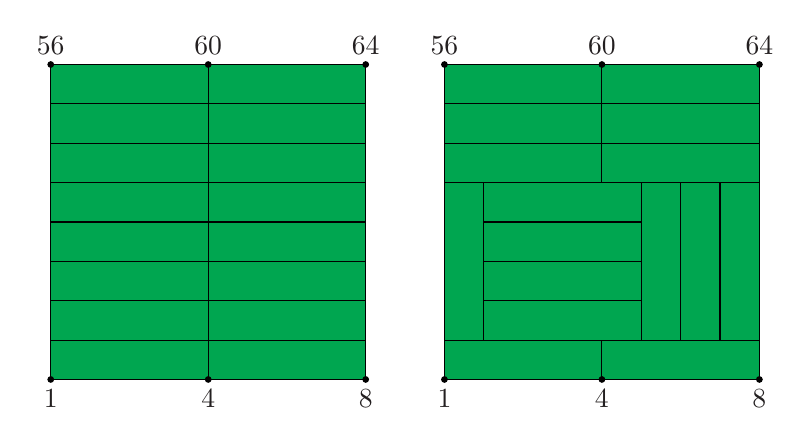
\begin{tikzpicture}[radius=0.1cm]
\selectcolormodel{cmyk}
\draw [fill=green] (0,0) rectangle (2,0.5);
\draw [fill=green] (2,0) rectangle (4,.5);
\draw [fill=green] (0,.5) rectangle (4,1);
\draw [fill=green] (2,.5) rectangle (4,1);
\draw [fill=green] (0,1) rectangle (2,1.5);
\draw [fill=green] (2,1) rectangle (4,1.5);
\draw [fill=green] (0,1.5) rectangle (2,2);
\draw [fill=green] (2,1.5) rectangle (4,2);

\draw [fill=green] (0,2) rectangle (2,2.5);
\draw [fill=green] (2,2) rectangle (4,2.5);
\draw [fill=green] (0,2.5) rectangle (2,3);
\draw [fill=green] (2,2.5) rectangle (4,3);
\draw [fill=green] (0,3) rectangle (2,3.5);
\draw [fill=green] (2,3) rectangle (4,3.5);
\draw [fill=green] (0,3.5) rectangle (2,4);
\draw [fill=green] (2,3.5) rectangle (4,4);

\draw [fill=green] (5,0) rectangle (7,.5);
\draw [fill=green] (7,0) rectangle (9,.5);

\draw [fill=green] (5,.5) rectangle (5.5,2.5);
\draw [fill=green] (5.5,.5) rectangle (7.5,1);
\draw [fill=green] (5.5,1) rectangle (7.5,1.5);
\draw [fill=green] (5.5,1.5) rectangle (7.5,2);
\draw [fill=green] (5.5,2) rectangle (7.5,2.5);
\draw [fill=green] (7.5,.5) rectangle (8,2.5);
\draw [fill=green] (8,.5) rectangle (8.5,2.5);
\draw [fill=green] (8.5,.5) rectangle (9,2.5);

\draw [fill=green] (5,2.5) rectangle (7,3);
\draw [fill=green] (7,2.5) rectangle (9,3);

\draw [fill=green] (5,3) rectangle (7,3.5);
\draw [fill=green] (7,3) rectangle (9,3.5);

\draw [fill=green] (5,3.5) rectangle (7,4);
\draw [fill=green] (7,3.5) rectangle (9,4);
\filldraw
(0,0) circle (1pt) node[align=left,   below] {1}
(2,0) circle (1pt) node[align=center, below] {4}
(4,0) circle (1pt) node[align=right,  below] {8} ;
\filldraw
(0,4) circle (1pt) node[align=left,  above] {56}
(2,4) circle (1pt) node[align=left,  above] {60}
(4,4) circle (1pt) node[align=left,  above] {64} ;
\filldraw
(5,0) circle (1pt) node[align=left,   below] {1}
(7,0) circle (1pt) node[align=center, below] {4}
(9,0) circle (1pt) node[align=right,  below] {8} ;
\filldraw
(5,4) circle (1pt) node[align=left,  above] {56}
(7,4) circle (1pt) node[align=left,  above] {60}
(9,4) circle (1pt) node[align=left,  above] {64} ;
\end{tikzpicture}
\end{center}

$$\left[\begin{array}{cccccccccccccccccc}
1 & 5 & 12 & 16 & 19 & 23 & 26 & 30 & 33 & 37 & 44 & 48 & 51 & 55 & 58 & 62\\
2 & 6 & 9 & 13 & 20 & 24 & 27 & 31 & 34 & 38 & 41 & 45 & 52 & 56 & 59 & 63\\
3 & 7 & 10 & 14 & 17 & 21 & 28 & 32 & 35 & 39 & 42 & 46 & 49 & 53 & 60 & 64\\
4 & 8 & 11 & 15 & 18 & 22 & 25 & 29 & 36 & 40 & 43 & 47 & 50 & 54 & 57 & 61
\end{array}\right]$$

$$\left[\begin{array}{cccccccccccccccccc}
1&5&33&12&19&26&37&30&23&16&44&48&51&55&58&62\\
2&6&9&13&20&27&34&38&31&24&41&45&52&56&59&63\\
3&7&17&10&21&28&35&14&39&32&42&46&49&53&60&64\\
4&8&25&11&18&29&36&22&15&40&43&47&50&54&57&61
\end{array}\right]$$

这里举例的两个角标矩阵是满足证明中的第一步的分组性质的。

通过计算机编程,可以验证定理中的部分结果如下:

\begin{align*}
&1 \times4,det(A) = pf^{4}(A) = 1^{4}=1\\
&4 \times4,det(A) = pf^{4}(A) = 2^{4}=16\\
&5 \times4,det(A) = pf^{4}(A) = 3^{4}=81\\
&6 \times4,det(A) = pf^{4}(A) = 4^{4}=256\\
&7 \times4,det(A) = pf^{4}(A) = 5^{4}=625\\
&8 \times4,det(A) = pf^{4}(A) = 7^{4}=2401\\
&8 \times3,det(A) = pf^{4}(A) = 1^{4}=1
\end{align*}
代码参考 \cite{IM}.
同时计算了一些不是4的倍数的情况:
\begin{align*}
&5 \times5,det(A) = pf^{4}(A) =0\\
&6 \times5,det(A) = pf^{4}(A) =0\\
&7 \times5,det(A) = pf^{4}(A) =0\\
\end{align*}
由上述证明定理自然推广为下述定理:

\begin{theorem}
\begin{equation}p_{i_{k}} \equiv k (mod 4) \end{equation},除$C_{r}*G_{4}$下标的元素外其余元素都为0,那么仍然有$$det(A)=pf^{4}(A)$$
\end{theorem}

\begin{theorem}\label{theorem_pf3}
将$1, \dots, n$分成四个个数相等的集合$S_{1},S_{2},S_{3},S_{4}$,
\begin{equation}p_{i_{1}} \in S_{1}, p_{i_{2}} \in S_{2}, p_{i_{3}} \in S_{3}, p_{i_{4}} \in S_{4}\end{equation}
\begin{equation}\label{bb}p_{1}<p_{5}<...<p_{N-3}\end{equation},满足性质的$C_{r}*G_{4}$元素以外其余都为0,那么仍然有$$det(A)=pf^{4}(A)$$
\end{theorem}
证明方法完全类似可以得到:
\begin{theorem}\label{theorem_pf4}
将$1, \dots, n$分成$2N$个相等的集合$S_{1},S_{2},\cdots,S_{2N}$,
\begin{equation}p_{i_{1}} \in S_{1}, p_{i_{2}} \in S_{2}, \cdots, p_{i_{2N}} \in S_{2N}\end{equation}
\begin{equation}\label{bb}p_{1}<p_{2N+1}<...<p_{n-2N+1}\end{equation},满足性质的$C_{r}*G_{2N}$元素以外其余都为0,那么仍然有$$det(A)=pf^{2N}(A)$$
\end{theorem}

尽管得到\ref{theorem_pf3},它还不够强,从形式上讲它还不是二维等式在四维下的自然推广。
回顾$\det(A)=pf^{2}(A)$的条件,
$$\alpha =\{(i_{1},j_{1}),(i_{2},j_{2}),\cdots ,(i_{n},j_{n})\}$$
$i_{k}<j_{k}$和$i_{1}<i_{2}<\cdots <i_{n}$
$${\displaystyle \pi _{\alpha }={\begin{bmatrix}1&2&3&4&\cdots &2n-1&2n\\i_{1}&j_{1}&i_{2}&j_{2}&\cdots &i_{n}&j_{n}\end{bmatrix}}}$$

下面给出一种自然泛化的推测:
$$\alpha =\{(i_{1},j_{1},k_{1},l_{1}),(i_{2},j_{2},k_{2},l_{2}),\cdots ,(i_{n},j_{n},k_{n},l_{n})\}$$
$i_{s}<j_{s}<k_{s}<l_{s}$和$i_{1}<i_{2}<\cdots <i_{n}$
$${\displaystyle \pi _{\alpha }={\begin{bmatrix}1&2&3&4&\cdots &4n-3&4n-2&4n-1&4n\\i_{1}&j_{1}&k_{1}&l_{1}&\cdots &i_{n}&j_{n}&k_{n}&l_{n}\end{bmatrix}}}$$
则
$$det(A)=pf^{4}(A)$$



在$4 \times 2$,\cite{VAL42}这个猜测是正确的,但是维数稍大一些,如$4 \times 3$,\cite{VAL34},$4 \times 4$,\cite{VAL44},则不成立。

从另外一方面,尝试将从属关系做一个变更,通过一些数据检验,得到如下猜测:
\begin{question}\label{guess_pf1}
将$1, \dots, n$分成两个个数相等的集合$S_{1},S_{2}$,
\begin{equation}p_{i_{1}} , p_{i_{3}} \in S_{1}, p_{i_{2}}, p_{i_{4}} \in S_{2}\end{equation}
\begin{equation}\label{bb}p_{1}<p_{5}<...<p_{N-3}\end{equation},满足性质的$C_{r}*G_{4}$元素以外其余都为0,那么$$det(A)$$在内维数为2*(2n)时为平方数,为2*(2n+1)时为负的平方数
\end{question}

\Thanks{感谢南京大学郭学军教授给予我相关的硕士论文开题,指导我研究的是关于多米诺骨牌覆盖的$2-adic$性质分析,但是在给出$2-adic$一些计算性质后,我却对此文中提出的泛化问题非常感兴趣,2010年至今已近十年,本人离开了大学校园,从事软件开发工作,一直在利用业余时间尝试将结论推广到更多维数的可能性,做了很多错误的尝试,如今终于有所突破,虽然本文结论还未和其他理论建立起联系,用途也不明确,但是结论比较理想的实现了本人最初的构想,甚感欣慰!尤其最近在计算时发现此种形式的矩阵在具有特殊形式时似乎行列式是负的平方数,感觉到和复数似乎有关联,如果能够在证明上有更大突破,对矩阵理论可能也将是一个重大丰富}

\BeginRef
\bibitem{Kly} P. W. Kasteleyn, The statistics of dimers on a lattice, {\it Physica.}, 1961, 27.
\bibitem{Kly2}  Kasteleyn, P. W. . "Dimer statistics and phase Transitions". Journal of Mathematical Physics. 4 (2): 287–293 1963.
\bibitem{KO} Richard Kenyon, Andrei Okounkov,  What is ... a dimer?, {\it Notices of the American Mathematical Society} MARCH 2005 VOLUME 52, NUMBER 3.

\bibitem{MA} Richard J. Mathar Paving rectangular regions with rectangular tiles: tatami and non-tatami tilings.{\it arXiv:1311.6135v1 [math.CO]},  24 Nov 2013

\bibitem{IM} \href{https://github.com/huih1984/Lattice-Tilings-and-Hyperdeterminant/blob/master/vc\%2B\%2B/high\%20dimension\%20matrix/IndexMatrix.cpp}{IndexMatrix}

\bibitem{VAL42} \href{https://github.com/huih1984/Lattice-Tilings-and-Hyperdeterminant/blob/master/vc\%2B\%2B/high\%20dimension\%20matrix/out_4_2_1.txt}{val42}
\bibitem{VAL34} \href{https://github.com/huih1984/Lattice-Tilings-and-Hyperdeterminant/blob/master/vc\%2B\%2B/high\%20dimension\%20matrix/out_3_4_1.txt}{val34}
\bibitem{VAL44} \href{https://github.com/huih1984/Lattice-Tilings-and-Hyperdeterminant/blob/master/vc\%2B\%2B/high\%20dimension\%20matrix/out_4_4_1.txt}{val44}

\EndRef

\end{document}
